\section{verification}
\label{sec:verification}

This chapter evaluates the performance and learning progression og the Deep Q-network 
(DQN)-based pokemon battle agent over two iteration. The objective of this analysis 
is to validate the effectiveness of the chosen algorithm and wether we have achieved
the desired results based on our reqirements. Performance is assessed through empirical
training results, including average rewards and win rates.  

\subsection{Methodology}
Over the 2 iterations, the verification process was conducted using the same hyperparameters
but using different formats of the pokemon battle environment.
The first iteration used a signle battle format with randomly selected pokemon each
episode, while the second iteration was trained using the VGC 2025 regulation G format.
Each version of the agent, was evaluated over a series of training episodes, and data 
was colledted for:
\begin{itemize}
    \item Average reward per interval of 10 episodes
    \item Win rate per interval of 10 episodes.
    \item Training loss (rolling averages)
\end{itemize}
The figures below illustrate the training process over time for:
\begin{itemize}
    \item Iteration 1 - Baseline model trained over 1000 episodes
    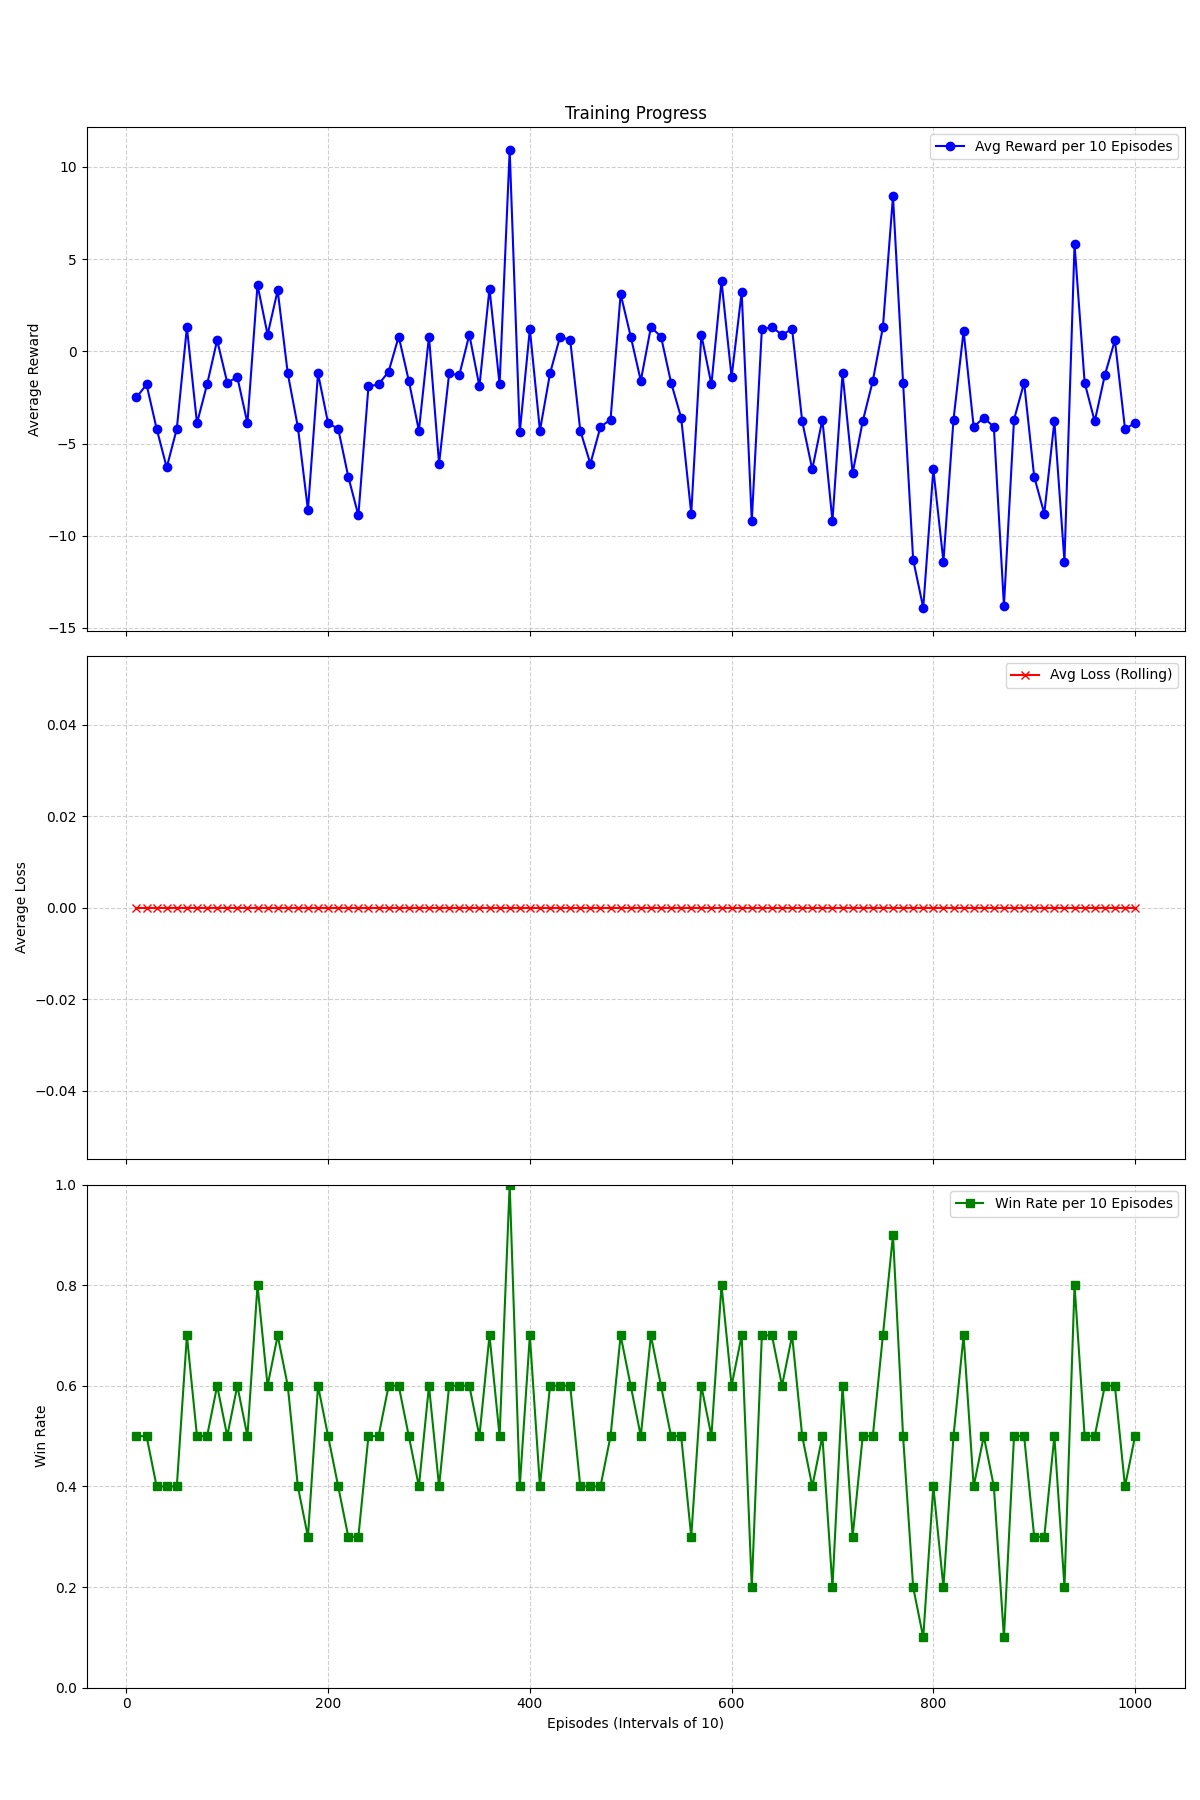
\includegraphics[width=.5]{assets/iteration-1-graphs.png}
    \item Iteration 2 - Enhanced model trained over 30000 episodes
    \includegraphics[width=.5]{}
\end{itemize}


\subsection{Results and analysis}
\textbf{Iteration 1 - Baseline model}
The first iteration exhibits very fluctuating performance, with relativly shallow 
state representation. Although the agent is capable of learning some degree of a control
policy, its reward curve is very erratic and lacks consistency.
